\section{复变函数期末练习题}

\subsection{习题 1}

\begin{figure}[H]
\centering
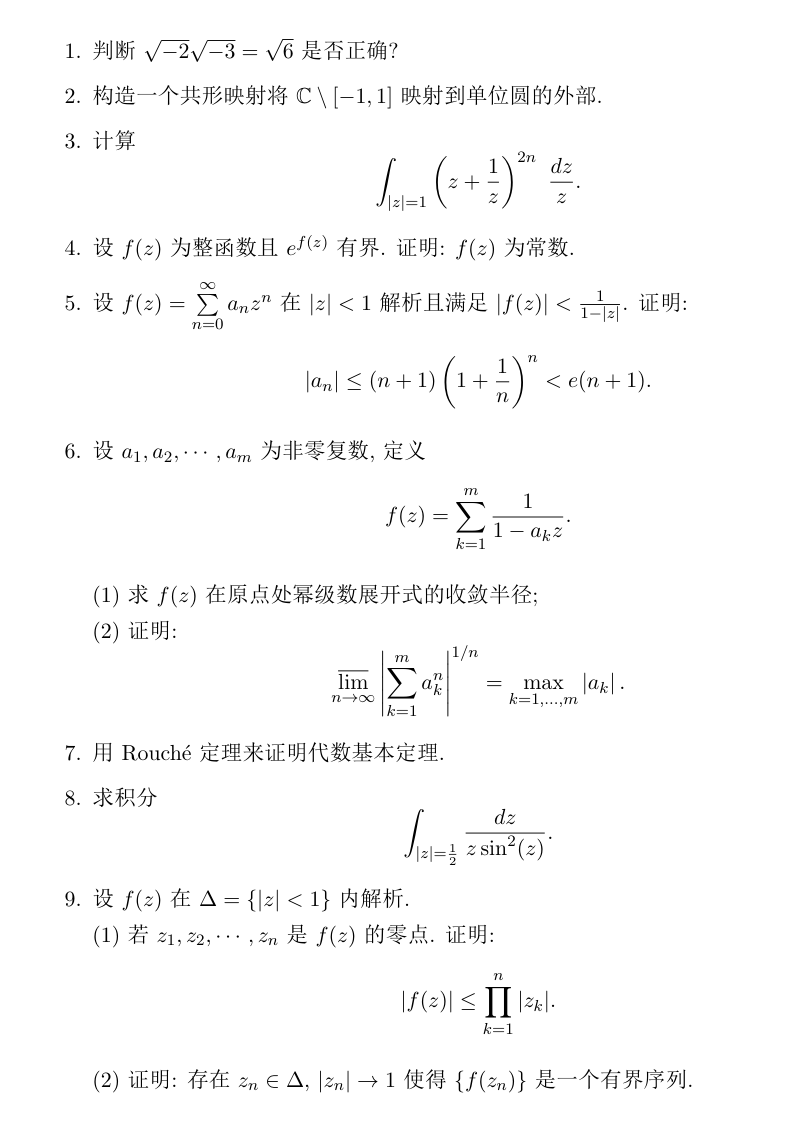
\includegraphics[width=\textwidth]{复变函数期末练习题-2025061100.png}
% \caption{}
\label{}
\end{figure}

\begin{enumerate}
	\item 错, $\sqrt{ -2 }\cdot \sqrt{ -3 }=\sqrt{ 2 }\cdot \sqrt{ -1 }\cdot \sqrt{ 3 }\cdot \sqrt{ -1 }=-\sqrt{ 6 }$.
	\item $w=\sqrt{ z^{2}-1 }+z$,其中 $\left.\sqrt{ z^{2}-1 }\right|_{z=i}=\sqrt{ 2 }i$.
	\item $f(z)\coloneqq\left( z+\frac{1}{z} \right)^{2n}\frac{1}{z}=\dots+\binom{2n}{n}z^{-1}+\dots$, $\int_{\lvert z \rvert=1}^{} f (z) \, \mathrm{d}z=\mathrm{res}_{0}f=2\pi i\binom{2n}{n}$.
	\item $e^{ f(z) }$ 也是整函数 (整函数 $e^{ z }$ 复合整函数 $f$) 于是 $e^{ f(z) }=C\Rightarrow f(z)=\log C$.
	\item $\lvert a_n \rvert=\left\lvert  \frac{1}{2\pi i}\int_{\lvert z \rvert=r}^{} \frac{f(z)}{z^{n+1}} \, \mathrm{d}z  \right\rvert\leq\frac{1}{r^{n}(1-r)}$,$r$ 待定,故可以取为 $\frac{n}{n+1}$,则 $\lvert a_n \rvert\leq(n+1)\left( 1+\frac{1}{n} \right)^{n}<e(n+1)$.
	\item $f(z)=\sum_{n=0}^{\infty}\left( \sum_{k=1}^{m}a_k^{n} \right)z^{n}$, 故 $R=\frac{1}{\varlimsup_{ n \to \infty }\sqrt[n]{ \left\lvert  \sum_{k=1}^{m}a_k^{n}  \right\rvert }}$. 同时 $R=\min_k\left\{  \left\lvert  \frac{1}{\lvert a_k \rvert}  \right\rvert  \right\}$ \footnote{一个函数在某点展开的幂级数,其收敛半径是从该点到离它最近的奇点的距离。}, 故 $\varlimsup_{ n \to \infty }\left\lvert  \sum_{k=1}^{m}a_k^{n}  \right\rvert ^{1/n }=\max_{k}\lvert a_k \rvert$.
	\item 归纳即可
	\item $f (z)\coloneqq \frac{1}{z\sin ^{2}z}$ 在 $\lvert z \rvert<\frac{1}{2}$ 内只有三阶极点 $0$,洛朗展开得到 $f(z)=\frac{1}{z\left( z-\frac{z^{3}}{3}+o(z^{4}) \right)^{2}}=\frac{1}{z^{3}}\cdot\frac{1}{\left( 1-\frac{z^{2}}{3}+o(z^{3}) \right)^{2}}=z^{-3}\cdot\frac{1}{1-\frac{2}{3}z^{2}+o(z^{3})}=z^{-3}+\frac{2}{3}z^{-1}+\dots$. 于是 $\mathrm{res}_{0}f=a_{-1}=\frac{2}{3}$. 故 $\int_{\lvert z \rvert<\frac{1}{2}}^{} f (z) \, \mathrm{d}z=2\pi i\mathrm{res}_{0}f=\frac{4}{3}\pi i$.
	\item 题目有误:应该补充条件 $\lvert f(z) \rvert<1$,且不等式改为 $\lvert f(0) \rvert\leq \prod_{k=1}^{n}\lvert z_k \rvert$.
	\begin{enumerate}
		\item 构造函数 $g(z)=\frac{f(z)}{\prod_{k=1}^{n}\varphi_{z_k}(z)}$,其中 $\varphi_{z_k}(z)\coloneqq\frac{z-z_k}{1-\overline{z_k}z}$. 于是 $\lvert z \rvert\to1$ 时,$\lvert \varphi_{z_k}(z) \rvert\to1$,故 $\lvert g(z) \rvert\to \lim_{ \lvert z \rvert \to 1 }\lvert f(z) \rvert\leq1$. 由最大模定理\footnote{最大模定理可以推广到趋于边界上,不需要在边界有定义,详见 Rudin p.253} $\lvert g (z) \rvert\leq1,\forall z\in \Delta$. 注意到 $\lvert \varphi_{z_k}(0) \rvert=\lvert z_k \rvert$,我们就有 $\lvert f(0) \rvert\leq\prod_{k=1}^{n}\lvert \varphi_{z_k}(0) \rvert=\prod_{k=1}^{n}\lvert z_k \rvert$.
		\item 反证而设,对于任意 $\{ \lvert z_k \rvert \}\to 1$, $\lvert f(z_k) \rvert\to \infty$. 接下来考虑 $f$ 在 $\Delta$ 内的零点个数,若为无穷个,这些零点存在聚点,则由非平凡解析函数的零点孤立性可知,聚点都在 $\partial\Delta$ 上,从而存在零点列 $\{ \lvert z_k \rvert \}\to1$,其中 $\lvert f(z_k) \rvert=0$,故 $\lvert f (z_k) \rvert \not\to \infty$. 故零点个数有限,按 (1) 中定义 $g$,则 $\frac{1}{g}\to 0$,在 $\lvert z \rvert\to1$ 时. $g\in H(\Delta)$ 无零点,故 $\frac{1}{g}\in H(\Delta)$ ,故由最大模定理:$\frac{1}{g}\equiv0$. $g$ 必须是无穷大,但这与 $g\in H(\Delta)$ 矛盾!
	\end{enumerate}
\end{enumerate}

\subsection{习题 2}

\begin{figure}[H]
\centering
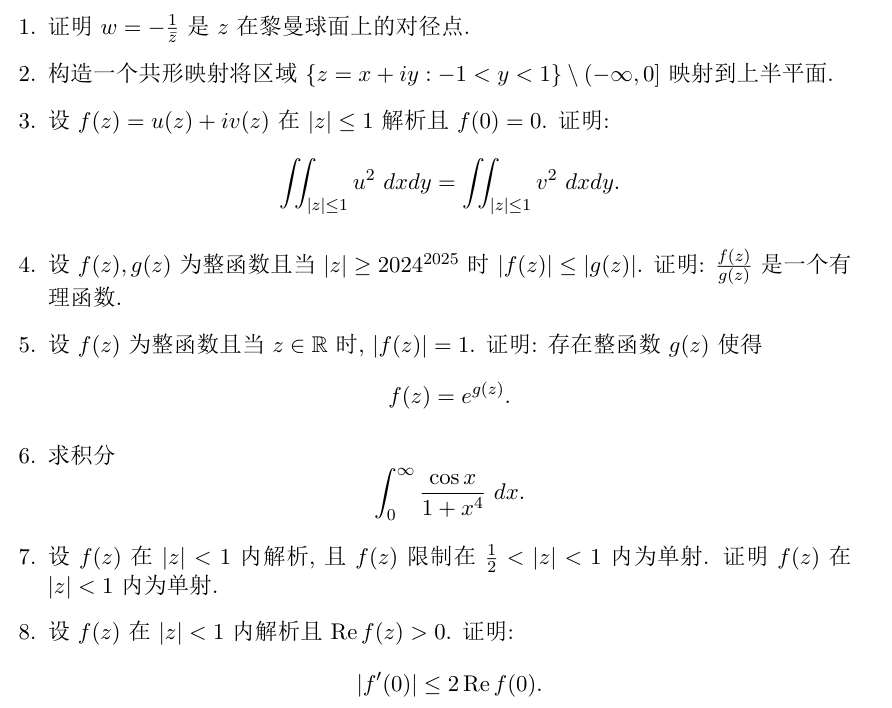
\includegraphics[width=\textwidth]{复变函数期末练习题-2025061109.png}
% \caption{}
\label{}
\end{figure}

\begin{enumerate}
	\item 映射 $\mathbb{C}\to S^{2},z=x+iy\mapsto\left( \frac{2x}{x^{2}+y^{2}+1},\frac{2y}{x^{2}+y^{2}+1},\frac{x^{2}+y^{2}-1}{x^{2}+y^{2}+1} \right)$. 而 $-\frac{1}{\overline{z}}=\frac{-x-iy}{x^{2}+y^{2}}\mapsto\left( \frac{-2x}{x^{2}+y^{2}+1},\frac{-2y}{x^{2}+y^{2}+1},\frac{-(x^{2}+y^{2}-1)}{x^{2}+y^{2}+1} \right)$, 于是是 $z$ 的对径点.
	\item $w=\sqrt{ 1-e^{ \pi z } }$.
	\item $\text{Re }f^{2}(z)=u^{2}-v^{2}$ 是调和函数,由平均值公式 $\int_{\lvert z \rvert<1}^{} u^{2}-v^{2} \, \mathrm{d}z=\pi \cdot1^{2}\cdot(u^{2}(0)-v^{2}(0))=0$.
	\item 记 $R=2024^{2025}$,在紧集 $\lvert z \rvert\leq R$ 内,由零点孤立性,$g$ 至多有有限个零点,$\frac{f}{g}$ 有有限个极点. 在 $\lvert z \rvert\geq R$ 上,$\lvert f(z) \rvert\leq \lvert g(z) \rvert\Rightarrow$ $g$ 的零点都是 $f$ 的零点, $\left\lvert  \frac{f}{g}  \right\rvert\leq1$ 有界,由黎曼可去奇点定理,$\frac{f}{g}$ 在该区域只有可去奇点. 且 $\frac{f}{g}$ 在无穷远点的邻域内有界,则 $\infty$ 不是本性奇点,只可能是可去奇点或极点. 因为任何在扩充复平面上亚纯的函数必然是有理函数,所以 $\frac{f}{g}$ 是有理函数.
	\item 还不确定,可以取 $g(z)=\int_{\gamma_{0\to z}}^{} \frac{f'(\zeta)}{f(\zeta)} \, \mathrm{d}\zeta+i\arg f(0)$,于是 $g'=\frac{f'}{f}$,故 验证这是整函数.
	\item $I=\frac{1}{2}\int_{-\infty}^{\infty} \frac{\cos x}{1+x^{4}} \, \mathrm{d}x$, 设 $f(z)=\frac{e^{ iz }}{1+z^{4}}$. 考虑在上半平面圆周上的积分,$\left\lvert  \int_{\gamma_{R}^{+}}^{} f(z) \, \mathrm{d}z  \right\rvert\to0$. 计算留数 $\mathrm{res}_{e^{ i\pi/4  }}f=\frac{1}{4}e^{ -1/\sqrt{ 2  } }e^{ i(1/\sqrt{ 2 }-3\pi/4 ) }$, $\mathrm{res}_{e^{ 3i\pi/4  }}f=\frac{1}{4}e^{ -1/\sqrt{ 2 } }e^{ i(-1/\sqrt{ 2 }-\pi/4 ) }$. 于是 $I=\frac{1}{2}\int_{-\infty}^{\infty} f (z) \, \mathrm{d}z=\pi i(\mathrm{res}_{e^{ i\pi/4  }}f+\mathrm{res}_{e^{ 3i\pi/4  }}f)=\frac{\pi}{2}e^{ -1/\sqrt{ 2 } }\sin\left( \frac{1}{\sqrt{ 2 }}+\frac{\pi}{4}  \right)$.
	\item 对于任意 $r\in\left( \frac{1}{2},1 \right)$, 考虑 $D_{r}$ 内 $f(z)=w_0$ 的解,$w_0$ 是任意复数,由于 $f$ 在 $C_{r}$ 上单射,故 $f(C_{r})$ 为简单闭曲线,由幅角原理,$N(w_0)=\frac{1}{2\pi i}\oint_{C_{r}}\frac{f'(z)}{f(z)-w_0}\mathrm{d}z$ 为 $f(C_{r})$ 在 $w_0$ 处的绕数,根据若当曲线定理,由于 $f(C_{r})$ 是简单闭曲线,那么对于任何不在 $f(C_{r})$ 上的 $w_0$,绕数为 0 或 1. 于是对于 $f(C_{r})$ 内部的 $w_0$,$f(z)-w_0=0$ 只有一个解.
	\item 定义 $g:\mathbb{D}\to \mathbb{D},z\mapsto\frac{f(z)-f(0)}{f(z)+\overline{f(0)}}$. 于是,$g(0)=0$, 由 Schwarz 引理,$\lvert g'(0) \rvert\leq1$,即 $\lvert f'(0) \rvert\leq2\text{Re }f(0)$.
\end{enumerate}

\subsection{习题 3}

\begin{figure}[H]
\centering
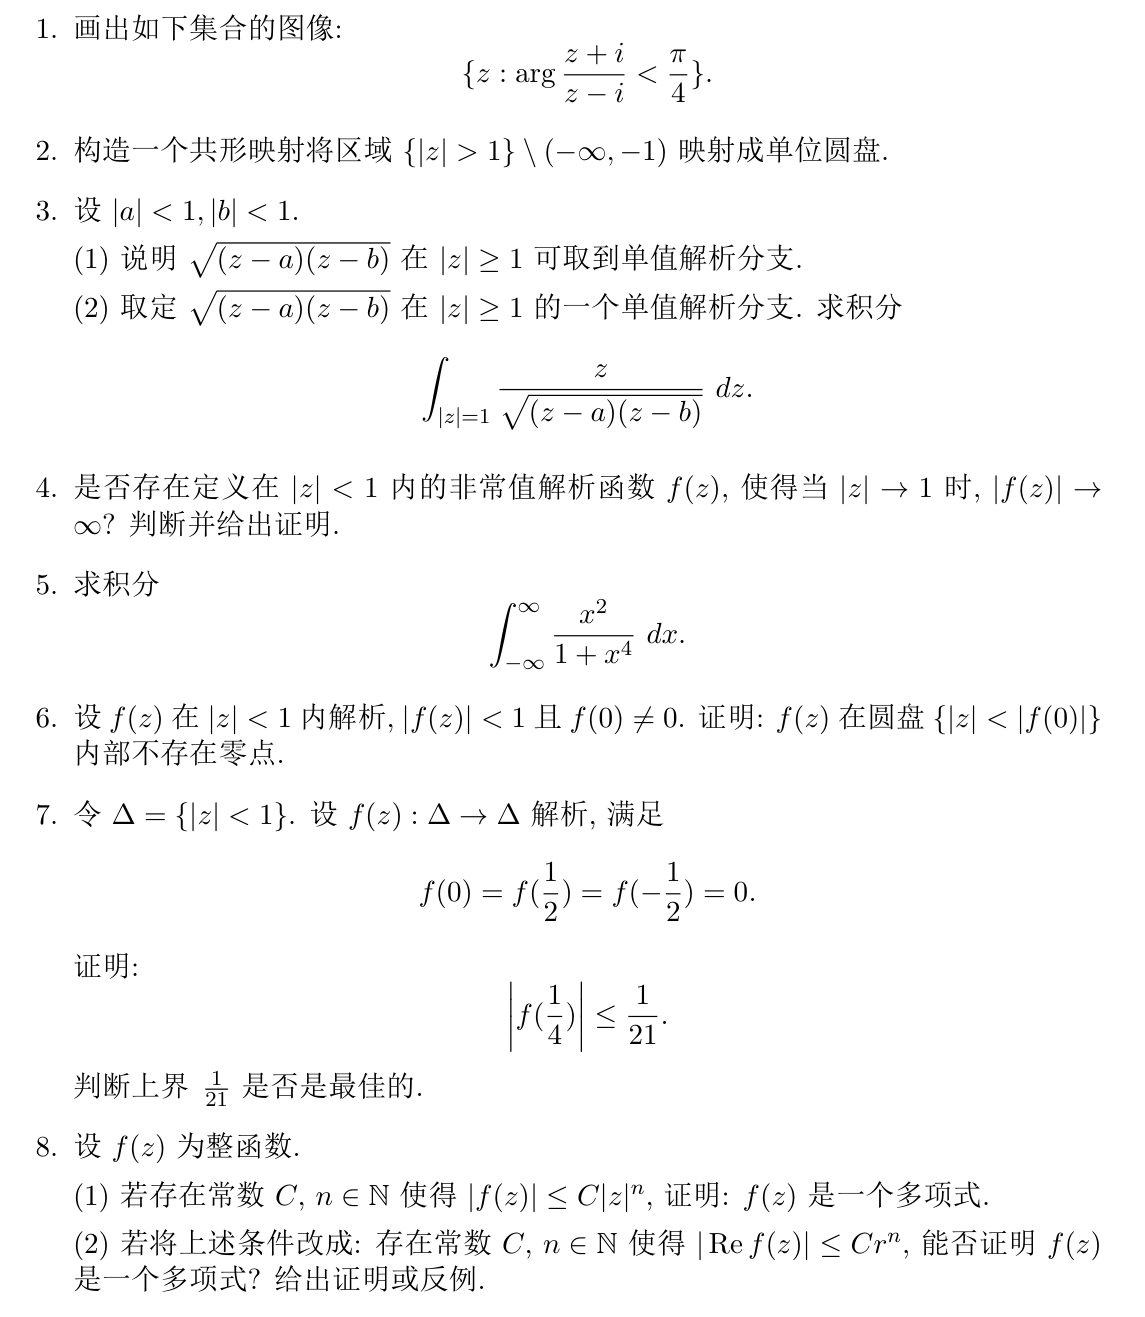
\includegraphics[width=\textwidth]{复变函数期末练习题-2025061121.png}
% \caption{}
\label{}
\end{figure}

\begin{enumerate}
	\item 这题很细节.
\begin{figure}[H]
\centering
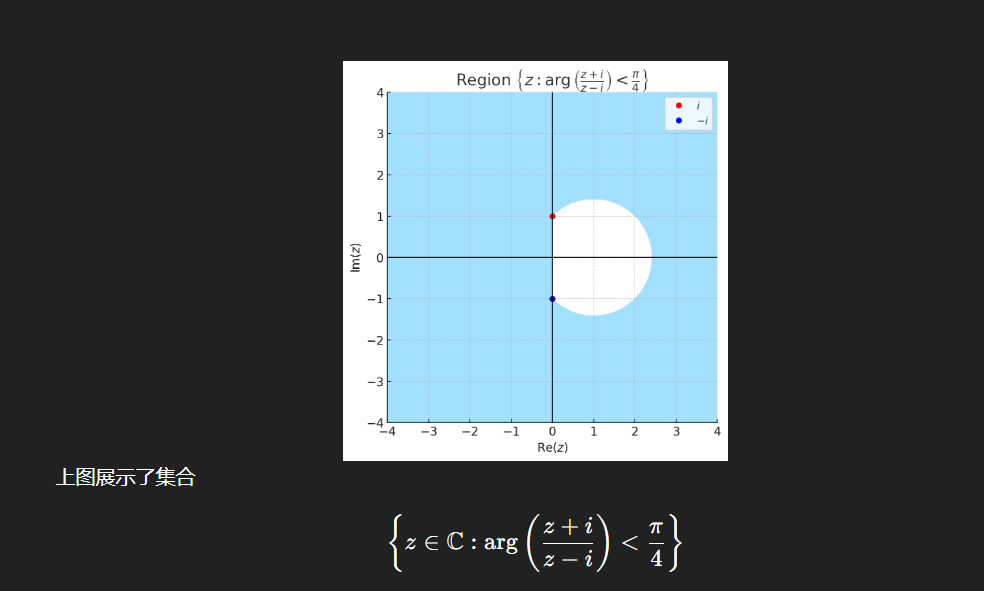
\includegraphics[width=\textwidth]{复变函数期末练习题-2025061911.png}
% \caption{}
\label{}
\end{figure}
	\item $\phi_1:\{ \lvert z \rvert>1 \}\setminus(-\infty,-1)\to \{ \text{Im }z>0;\lvert z \rvert>1 \},z\mapsto \sqrt{ -z }$. $\phi_2:\{ \text{Im }z>0;\lvert z \rvert>1 \}\to \{ \text{Im }z>0 \},z\mapsto z+\frac{1}{z}$. $\phi_3:\{ \text{Im }z>0 \}\to \{ \lvert z \rvert<1 \},z\mapsto\frac{z-i}{z+i}$. 于是 $\phi=\phi_3\circ \phi_2\circ \phi_1:\{ \lvert z \rvert>1 \}\setminus(-\infty,-1)\to \{ \lvert z \rvert<1 \},z\mapsto\frac{z-\sqrt{ z }-1}{z+\sqrt{ z }-1}$.
	\item (1) $f$ 在 $\{ \lvert z \rvert\geq1 \}$ 内没有支点,所以可以取单值分支. (2) 计算在 $a,b$ 处的留数 ($a_{-1}$) 得到 $I=\pi i(a+b)$.
	\item 不存在. 若存在,则由非常数的解析函数的零点孤立性,$f$ 只可能在 $\mathbb{D}$ 内有有限多个零点 $z_1,\dots,z_n$. 考虑 $g (z)\coloneqq\frac{f (z)}{\prod_{k=1}^{n}\varphi_{z_k}(z)}\in H(\mathbb{D})$,且在 $\mathbb{D}$ 内没有零点,于是 $\frac{1}{g}\in H(\mathbb{D})$. 令 $\lvert z \rvert\to1$,我们有 $\lvert \varphi_{z_k}(z) \rvert\to1,\lvert f(z) \rvert\to \infty$,于是 $\left\lvert  \frac{1}{g}  \right\rvert\to0$. 由最大模原理\footnote{见 Rudin},$\max_{\lvert z \rvert<1}\left\lvert  \frac{1}{g(z)}  \right\rvert\leq0$. 于是 $\frac{1}{g}=0$,$g$ 在 $\mathbb{D}$ 内处处取到无穷,这与 $g\in H(\mathbb{D})$ 矛盾!
	\item 记 $f(z)=\frac{z^{2}}{1+z^{4}}$,考虑在上半圆周上积分,在圆弧上积分趋于 0,计算围道内留数:$\mathrm{res}_{e^{ \pi i/4  }}f=\frac{1-i}{4\sqrt{ 2 }}$, $\mathrm{res}_{e^{ 3\pi i/4  }}f=\frac{-1-i}{4\sqrt{ 2 }}$. 于是 $I=2\pi i(\mathrm{res}_{e^{ \pi i/4  }}f+\mathrm{res}_{e^{ 3\pi i/4  }}f)=\frac{\pi}{\sqrt{ 2 }}$.
	\item 若存在 $\lvert \alpha \rvert<\lvert f(0) \rvert$ 使得 $f(\alpha)=0$,利用 Schwarz-pick lemma,$\left\lvert  \frac{f (b)-f (a)}{1- \overline{f (a)}f (b)}  \right\rvert\leq \left\lvert  \frac{b-a}{1-\overline{a}b}  \right\rvert,\forall a, b\in \mathbb{D}$, 取 $a=\alpha,b=0$,就有 $\lvert f(0) \rvert\leq \lvert \alpha \rvert$,矛盾!
	\begin{itemize}
		\item 证明 Schwarz-pick lemma:令 $\varphi_{a}(z)\coloneqq\frac{a-z}{1-\overline{a}z}$,对于 $f:\mathbb{D}\to \mathbb{D}$,考虑 $\varphi_{f(a)}\circ f\circ\varphi_{a}:\mathbb{D}\to \mathbb{D}$,它将 0 映射到 0,于是由 Schwarz 引理,$\lvert \varphi_{f(a)}(f(\varphi_{a}(z))) \rvert\leq \lvert z \rvert$,取 $z=\varphi_{a}(b)$,则 $\lvert \varphi_{f(a)}(f(b)) \rvert\leq \lvert \varphi_{a}(b) \rvert$, 即 $\left\lvert  \frac{f(a)-f(b)}{1-\overline{f(a)}f(b)}  \right\rvert\leq \left\lvert  \frac{a-b}{1-\overline{a}b}  \right\rvert$.
	\end{itemize}
	\item 记 $\varphi_{a}(z)\coloneqq\frac{a-z}{1-\overline{a}z}$,考虑 $g(z)\coloneqq\frac{f(z)}{\varphi_{0}(z)\cdot\varphi_{1/2}(z)\cdot\varphi_{-1/2}(z)}$,由于 $f\in H(\Delta)$ 在 $0,\frac{1}{2},-\frac{1}{2}$ 有零点,则 $g\in H(\Delta)$. 因为 $\lvert f(z) \rvert<1$,所以 $\lvert z \rvert\to1$ 时,$\lvert g(z) \rvert\to \lim_{ \lvert z \rvert \to 1 }\lvert f(z) \rvert\leq1$. 于是由最大模原理\footnote{只需要趋于边界时的最大值即可,见 Rudin p.253},$\max_{z\in\Delta}\lvert g(z) \rvert\leq1$. 令 $z=\frac{1}{4}$,就有 $\left\lvert  g\left( \frac{1}{4} \right)  \right\rvert=\frac{\left\lvert  f\left( \frac{1}{4} \right)  \right\rvert}{\left\lvert  \left( -\frac{1}{4} \right)\cdot\left( \frac{2}{7} \right)\cdot\left( -\frac{2}{3} \right)  \right\rvert}=21\left\lvert  f\left( \frac{1}{4} \right)  \right\rvert\leq1$,即 $\left\lvert  f\left( \frac{1}{4} \right)  \right\rvert\leq\frac{1}{21}$. 这是最佳上界,因为等号成立当且仅当 $g\equiv1$,也就是 $f(z)=\varphi_{0}(z)\varphi_{1/2 }(z)\varphi_{-1/2 }(z)$.
	\item (1) $f\in H(\mathbb{C})$ 可写作 $f(z)=\sum_{k=0}^{\infty}a_kz^{k}$,由 Cauchy 积分公式,$a_k=\frac{1}{2\pi i}\int_{\lvert z \rvert=R}^{} \frac{f(z)}{z^{k+1}} \, \mathrm{d}z$,于是 $\lvert a_k \rvert\leq\frac{1}{2\pi}\int_{\lvert z \rvert=R}^{} \frac{\lvert f(z) \rvert}{\lvert z \rvert ^{k+1}} \, \lvert \mathrm{d}z \rvert\leq\frac{1}{2\pi}\int_{\lvert z \rvert=R}^{} \frac{C}{\lvert z \rvert ^{k+1-n}} \, \lvert \mathrm{d}z \rvert\leq\frac{C}{R^{k-n}}$. 当 $k>n$ 时,由 $R$ 的任意性,令 $R\to \infty$,则 $a_k=0$. 于是 $f$ 是一个至多 $n$ 次多项式. (2) 利用 Borel-Carathéodory Theorem,对于 $\lvert z \rvert\leq r$,$\lvert f(z) \rvert\leq\frac{2r}{R-r}\max_{\lvert \zeta \rvert=R}(\text{Re }f(\zeta))+\frac{R+r}{R-r}\lvert f(0) \rvert$,其中 $0<r<R$. 取 $R=2r$. 于是 $\lvert f(z) \rvert\leq C'\lvert z \rvert ^{n}+D$,其中 $C',D$ 是与 $z$ 无关的常数. 类似 (1) 的讨论可知 $f$ 是多项式.
	\begin{itemize}
		\item Borel-Carathéodory Theorem 的证明:
		\item \begin{figure}[H]
\centering
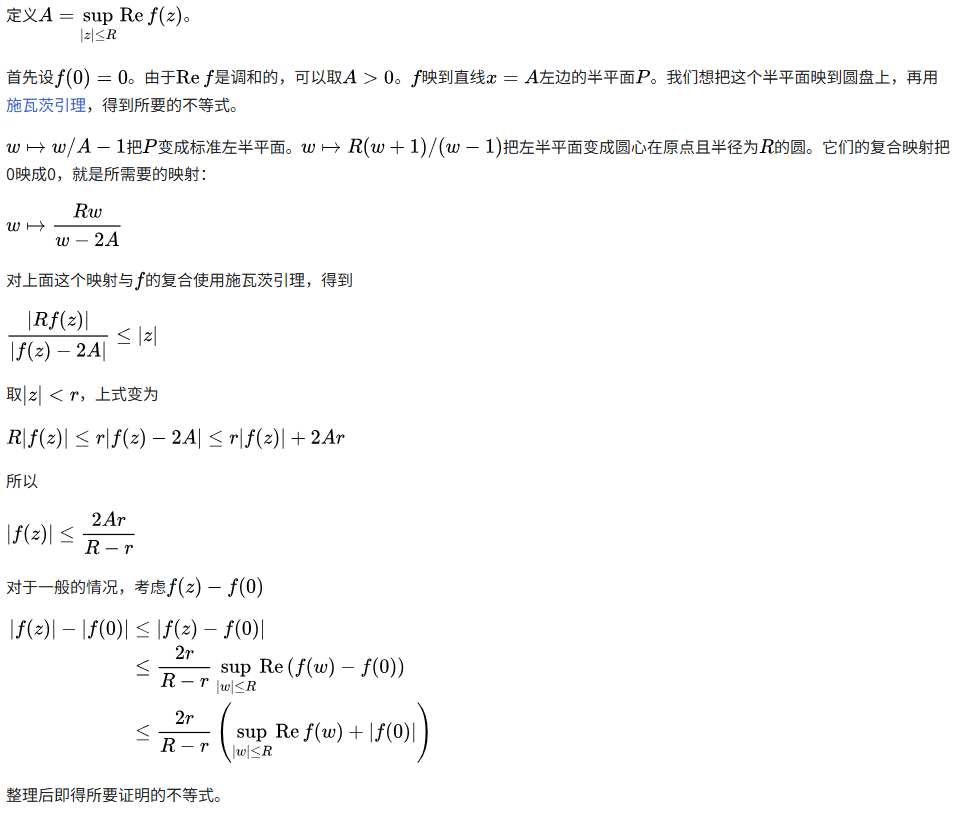
\includegraphics[width=\textwidth]{复变函数期末练习题-2025061123.png}
% \caption{}
\label{}
\end{figure}
	\end{itemize}
\end{enumerate}
